\section{Qualità di processo}

\subsection{Introduzione}

Nello svolgimento del progetto, i processi fanno uso di criteri di qualità, attraverso i quali è possibile perseguire un miglioramento continuo che porti alla più completa soddisfazione di questi criteri. In questo progetto, si è scelto di fare uso del metodo PDCA e dello standard ISO/IEC 15504 (SPICE). Attraverso \glock{PDCA} e \glock{SPICE}, è possibile garantire uno svolgimento dei processi che tendono, attraverso l'esperienza, a migliorarsi e ad assicurare al cliente l'ottenimento di un prodotto di qualità.
In questa sezione si espongono i livelli di qualità accettabili e ottimali sulla base delle metriche scelte all'interno del documento \dext{Norme di Progetto v1.0.0}.

\subsection{Monitoraggio dei processi}

I processi monitorati con delle metriche precise di qualità sono i seguenti:

\begin{itemize}
	\item QP-1. Gestione delle risorse;
	\item QP-2. Gestione dei rischi.
 	\item QP-3. Analisi dei Requisiti
	\item QP-4. Verifica del software
\end{itemize}

	\subsubsection{QP-1. Gestione delle risorse}

		Il processo di gestione delle risorse si riserva di gestire la copertura delle risorse disponibili e delle attività schedulate all'interno del \dext{Piano di Progetto v1.0.0}. Di seguito vengono esposte le metriche utilizzate, che possono essere visionate all'interno del documento \dext{Norme di Progetto v1.0.0}.

		\paragraph{Metriche utilizzate}

			\begin{itemize}
				\item QM-PROC-1. Budgeted Cost of Work Scheduled (BCWS);
				\item QM-PROC-2. Actual Cost of Work Performed (ACWP);
				\item QM-PROC-3. Budgeted Cost of Work Performed (BCWP);
				\item QM-PROC-4. Schedule Variance (SV);
				\item QM-PROC-5. Cost Variance (CV).
			\end{itemize}

		\paragraph{Indici di qualità}

			\begin{center}
				\rowcolors{2}{white}{lightest-grayest}
				\begin{longtable}{|c|c|c|}
				\hline
				\rowcolor{lighter-grayer}
				\textbf{ID metrica} & \textbf{Valore preferibile} & \textbf{Valore accettabile}\\
				\hline
				\endfirsthead
				\hline
				QM-PROC-1 (BCWS) & // & // \\
				\hline
				QM-PROC-2 (ACWP) & // & // \\
				\hline
				QM-PROC-3 (BCWP) & // & // \\
				\hline
				QM-PROC-4 (SV) & \(0\%\) & \(\ge -5\%\) \\
				\hline
				QM-PROC-5 (CV) & \(0\%\) & \(\ge -5\%\) \\
				\hline
				\caption{Indici di qualità per le metriche di gestione delle risorse}
				\end{longtable}
			\end{center}

	\subsubsection{QP-2. Gestione dei rischi}

		Il processo di gestione dei rischi monitora la comparsa di nuovi rischi che possono avvenire durante le fasi del progetto.
		Per ogni fase del progetto si eseguirà una relativa analisi retrospettiva dei rischi precedentemente segnalati e, in caso di nuovi rischi, si cercherà di risolverli nel minor tempo possibile.
		Di seguito vengono esposte le metriche utilizzate, che possono essere visionate all'interno del documento \dext{Norme di Progetto v1.0.0}.

		\paragraph{Metriche utilizzate}

			\begin{itemize}
				\item QM-PROC-6. Unbudgeted Risks (BCWS).
			\end{itemize}

		\paragraph{Indici di qualità}

			\begin{center}
				\rowcolors{2}{white}{lightest-grayest}
				\begin{longtable}{|c|c|c|}
				\hline
				\rowcolor{lighter-grayer}
				\textbf{ID metrica} & \textbf{Valore preferibile} & \textbf{Valore accettabile}\\
				\hline
				\endfirsthead
				\hline
				QM-PROC-6 (UR) & \(0 \text{rischi}\) & \(\le 5 \text{rischi}\) \\
				\hline
				\caption{Indici di qualità per le metriche di gestione dei rischi}
				\end{longtable}
			\end{center}

			Di seguito il grafico che rappresenta i rischi non preventivati per il periodo di analisi dei requisiti:

			\begin{figure}[H]
				\centering
				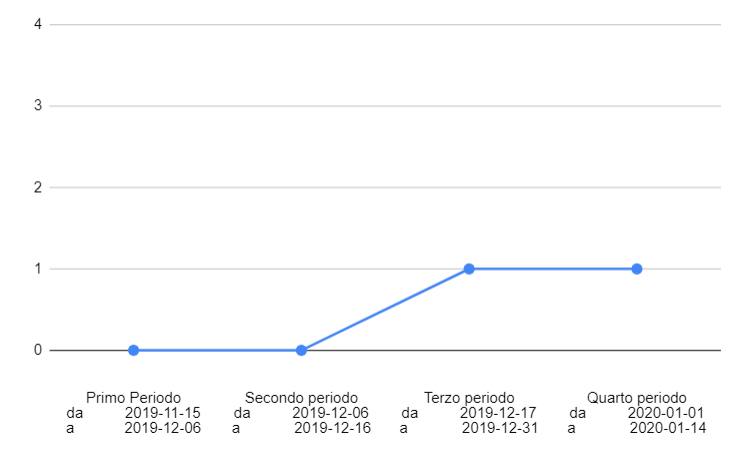
\includegraphics[width=0.8\linewidth]{./res/images/rischi.png}
				\caption{Grafico periodo/rischio nel periodo di analisi dei requisiti}
				\label{fig:Grafico periodo/rischio nel periodo di analisi dei requisiti}
			\end{figure}

	\subsubsection{QP-3. Analisi dei Requisiti}

		Il processo di Analisi dei Requisiti vuole tenere traccia di tutti i requisiti portati a termine fino alla data corrente e dell'eventuale valore aggiunto che possono costituire i requisiti non obbligatori.
		Di seguito vengono esposte le metriche utilizzate, che possono essere visionate all'interno del documento \dext{Norme di Progetto v1.0.0}.

		\paragraph{Metriche utilizzate}

			\begin{itemize}
				\item QM-PROC-7. Satisfied Mandatory Requirements (SMR)
				\item QM-PROC-8. Satisfied Desirable Requirements (SDR)
				\item QM-PROC-9. Satisfied Optional Requirements (SOR)
			\end{itemize}


		\paragraph{Indici di Qualità}

			\begin{center}
				\rowcolors{2}{white}{lightest-grayest}
				\begin{longtable}{|c|c|c|}
				\hline
				\rowcolor{lighter-grayer}
				\textbf{ID Metrica} & \textbf{Valore Preferibile} & \textbf{Valore Accettabile}\\
				\hline
				\endfirsthead
				\hline
				QM-PROC-7 (SMR) & \(\geq 100\%\) & \(\geq 100\%\) \\
				\hline
				QM-PROC-8 (SDR) & \(\geq 50\%\) & \(\geq 15\%\) \\
				\hline
				QM-PROC-9 (SOR) & \(\geq 15\%\) & \(\geq 0\%\) \\
				\hline
				\caption{Indici di qualità per le metriche di Analisi dei Requisiti}
				\end{longtable}
			\end{center}

	\subsubsection{QP-4. Verifica del Software}

		Il processo di Verifica del Software pone come obiettivo il controllo dello sviluppo software a livello di codifica.
		Di seguito vengono esposte le metriche utilizzate, che possono essere visionate all'interno del documento \dext{Norme di Progetto v1.0.0}.

		\paragraph{Metriche utilizzate}

			\begin{itemize}
				%NDR: da usare dopo
				\item QM-PROC-10. Branch Coverage (BCOV)
				\item QM-PROC-11. Condition Coverage (COCOV)
				\item QM-PROC-12. Statement Coverage (SCOV)
				\item QM-TEST-1. Passed Test Cases Percentage (PTCP)
				\item QM-TEST-2. Failed Test Cases Percentage (FTCP)
				\item QM-TEST-3. Bug-Fixing Percentage (BFP)
				\item QM-TEST-4. Test Effectiveness (TE)
			\end{itemize}


		\paragraph{Indici di Qualità}

			\begin{center}
				\rowcolors{2}{white}{lightest-grayest}
				\begin{longtable}{|c|c|c|}
				\hline
				\rowcolor{lighter-grayer}
				\textbf{ID Metrica} & \textbf{Valore Preferibile} & \textbf{Valore Accettabile}\\
				\hline
				\endfirsthead
				\hline
				QM-PROC-10 (BCOV) & \(\geq 75\%\) & \(\geq 50\%\) \\ \hline
				QM-PROC-11 (COCOV) & \(\geq 50\%\) & \(\geq 25\%\) \\ \hline
				QM-PROC-12 (SCOV) & \(\geq 75\%\) & \(\geq 50\%\) \\ \hline
				QM-TEST-1 (PTCP) & \(\geq 100\%\) & \(\geq 100\%\) \\ \hline
				QM-TEST-2 (FTCP) & \(\geq 0\%\) & \(\geq 0\%\) \\ \hline
				QM-TEST-3 (BFP) & \(\geq 100\%\) & \(\geq 100\%\) \\ \hline
				QM-TEST-4 (TE) & \(\geq 75\%\) & \(\geq 50\%\) \\ \hline
				\hline
				\caption{Indici di qualità per le metriche di Verifica del Software}
				\end{longtable}
			\end{center}
